\section{Related Works}
Currently, numerous recommend systems have been developed to provide laptop suggestions tailored to user needs. These systems illustrate different approaches to handling user requirements, ranging from content-based and collaborative filtering methods to ontology-based models. As a result, a considerable body of prior research exists in this domain, offering valuable insights and serving as important references for ongoing and future studies.



~\textcite{bahramian2015} developed an ontology-based tourism recommend system that applied a spreading activation model to enhance personalization. Their system represented both user preferences and points of interest (POIs) through an ontology, dynamically adapted recommendations with feedback, and addressed cold-start and sparsity problems. The results showed improved diversity and relevance in recommendations.

~\textcite{ayundhita2019} investigated a laptop recommend system using an Ontology-Based Conversational Recommend System (CRS). Their approach integrated ontological reasoning with interactive questioning to capture user requirements more effectively. Experimental evaluation showed that the system achieved an accuracy of 84.6\% when tested with functionality requirement questions.


~\textcite{putra2024} proposed a hybrid laptop recommend system that combined ontology-based filtering with collaborative filtering in a conversational framework. The ontology component mapped functional requirements to technical specifications, while collaborative filtering introduced diversity by leveraging similar user preferences. Their system achieved 93.33\% accuracy, outperforming earlier ontology-only approaches.

Based on previous studies, we will develop an ontology-based recommend system incorporating the Collaborative Filtering (CF) method to recommend laptops based on daily user needs.

\begin{flushleft}
	\textbf{Ontology-Based Recommend System}
\end{flushleft}

An ontology-based recommend system is a type of recommend system that utilize ontology - formal representations of knowledge within a specific domain. Such systems are particularly advantageous in domains like the Semantic Web (SW), Artificial Intelligence (AI), and Systems Engineering (SE), where complex relationship must be analyzing and modeling.
Implementing  an  Ontology-Based  Recommend  system  involves  developing  an  ontology  related  to  a particular domain or topic, involving concepts, relations, and rules. Researchers evaluate the similarity between user preferences and ontology by using it to model user preferences

\begin{flushleft}
	\textbf{Collaborative Filtering}
\end{flushleft}
Recommend system provides personalize recommendations to users base on their interest. One of most popular type of such system is Collaborative Filtering (CF), operating the prediction based on the known user ratings of items ~\parencite{zhang2014}. Collaborative filtering techniques generate recommendations by analyzing user behavior patterns, without relying on external information about items or users ~\parencite{Koren2022}.

In collaborative filtering, user similarity is commonly assessed through advanced measures such as cosine similarity and Pearson correlation, which enable detailed analysis of shared preferences. Conversely, item-based collaborative filtering identifies items with attributes resembling those that a user has previously valued or interacted with. In this approach, similarity between items is computed from user interaction patterns, thereby enhancing the depth of preference modeling and supporting the generation of more relevant recommendations.

Although this approach is strong for most case, some users may find it difficult to get their satisfied recommendations due to their unique desire. Furthermore, the cold-start problem presents a significant challenge, as new users or items lack sufficient historical data to generate accurate recommendations. Therefore, it is essential to combine multiples techniques to accomplish decent accuracy and effectiveness for recommend system.

\begin{flushleft}
	\textbf{Conversational Recommend System}
\end{flushleft}
A conversational recommend system(CRS) is an interactive software designed to help users navigate effectively through the items and make recommendations by identifying their needs through feedback mechanisms~\parencite{inproceedings}. At present, CRS can be classified into two categories: those that emphasize an item’s technical specifications and those that prioritize its functionality~\parencite{ayundhita2019}.

Technical specification approach focus on characteristics of items, such as weight, color, material. While functionality approach operating on the benefits, or functions of items. Both are required to interact with users to gain theirs feedback to provide accurate and effective recommendations.

\begin{flushleft}
	\textbf{Ontology design}
\end{flushleft}
Below is our proposed ontology-design based on RDF/OWL standard and ontology building using Protégé software. In ontology-building, four main components are involved: classes, property objects, data properties, and individuals. Figure 1 show the comprehensive ontology design with 4 main classes: Functionality, PriceRange, Product, Specification:

\begin{figure}[htbp]
	\centering
	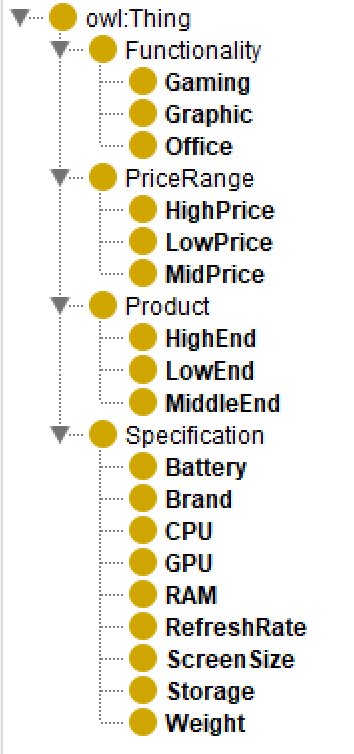
\includegraphics[width=0.33\textwidth]{ontology-design.png}
	\caption{Ontology design with 4 main classes}
	\label{fig:sample}
\end{figure}

The Functionality class used to organize laptops into different functional requirements by users, this class organize laptops into 3 sub-classes: Gaming, Graphic, Office.

The Product class organizes laptops into different products tier, including HighEnd laptops, MiddleEnd laptops, and Lowend laptops.

The Specification is used to organize product specifications in the laptops domain. This class has the purpose of mapping functional requirements and price range of laptop with coresponding laptop.

\begin{flushleft}
	\textbf{User Preference Modelling}
\end{flushleft}
User preference modeling plays a critical role in recommender systems~\parencite{ayundhita2019}. Its primary aim is to formulate appropriate questions and construct user profiles from the feedback provided. Through various data processing techniques, researchers are able to capture and analyze user preferences more precisely, thereby facilitating a deeper understanding of user needs. Commonly discussed cases include the following:

\begin{enumerate}[label=\alph*)]
	\item \textbf{Empty User.} This case arises when no user profile has been established and there is no available information regarding the user’s preferences or needs. The recommended strategy is to initiate the interaction by posing preliminary questions and gradually constructing the user profile~\parencite{ayundhita2019}.  
	
	\item \textbf{Abundance of Product Choices.} This situation occurs when users are presented with a wide range of products, making the decision process more time-consuming. In such cases, users may opt for multiple recommendations. The suggested strategy involves asking questions that emphasize the distinguishing features of each product~\parencite{ayundhita2019}.  
	
	\item \textbf{Absence of Suitable Recommendations.} Here, users struggle to identify a product that meets their functional requirements. The proposed solution is to first elicit functional requirements at the current level and then revisit any unmet operational requirements from the previous level~\parencite{ayundhita2019}.  
	
	\item \textbf{Unmet Requirements.} This case highlights situations where the initial requirement definitions fail to produce appropriate recommendations. The strategy involves refining the inquiry by requesting more specific functional requirements at the next level~\parencite{ayundhita2019}.  
	
	\item \textbf{No Product Matches the User Profile.} In this scenario, the defined requirements are insufficient to generate relevant recommendations. The proposed approach is to revise the requirements and request more specific functional details at the next level~\parencite{ayundhita2019}.  
\end{enumerate}

